\documentclass[11pt]{article}

% ---- Packages ----
\usepackage[utf8]{inputenc}
\usepackage[T1]{fontenc}
\usepackage{amsmath,amssymb}
\usepackage{graphicx}
\usepackage{booktabs}
\usepackage{hyperref}
\usepackage{natbib}
\usepackage[margin=1in]{geometry}
\usepackage{microtype}
\usepackage{lineno}
\linenumbers

% ---- Title ----
\title{BELA: A Fully Automated Blastocyst Evaluation Learning Algorithm for Ploidy Prediction from Time-Lapse Imaging}
\date{}

\begin{document}
\maketitle

% ==========================================================================
% ABSTRACT
% ==========================================================================
\begin{abstract}
Accurate assessment of embryo ploidy status is a central challenge in assisted reproduction, yet the prevailing approach---preimplantation genetic testing for aneuploidy (PGT-A)---requires an invasive trophectoderm biopsy and is susceptible to errors arising from embryonic mosaicism. Image-based deep learning models offer a non-invasive alternative, but existing systems either depend on subjective embryologist annotations or underutilize the temporal information captured by time-lapse imaging platforms. Here we present BELA (Blastocyst Evaluation Learning Algorithm), a two-step automated pipeline that first predicts blastocyst quality scores from day-5 time-lapse sequences (96--112 hours post insemination) using a multitask bidirectional long short-term memory network and then combines the model-derived blastocyst score with maternal age in a logistic regression to classify ploidy status. On the Weill Cornell Medicine Embryoscope test set, BELA achieves an area under the receiver operating characteristic curve (AUC) of $0.76 \pm 0.002$ for distinguishing euploid from aneuploid embryos and $0.826 \pm 0.004$ for distinguishing euploid from complex aneuploid embryos when maternal age is included, matching or exceeding models that require embryologist-derived scores. External validation across four datasets comprising 4{,}251 embryos from three clinics and two imaging instruments confirms that BELA consistently outperforms day-5 video baselines ($p < 0.05$). By removing the need for subjective manual annotation, BELA provides an objective, reproducible, and deployable tool---available through the web-based STORK-V platform---for embryo evaluation in clinical IVF practice.
\end{abstract}

% ==========================================================================
% INTRODUCTION
% ==========================================================================
\section{Introduction}

Since its inception in 1978, in vitro fertilization (IVF) has enabled over eight million births worldwide and remains the principal treatment for couples who cannot conceive naturally. The success of each IVF cycle depends critically on the selection of a single high-quality embryo for transfer, because transferring multiple embryos to compensate for uncertain selection carries an elevated risk of multiple pregnancies and their associated complications. At the core of embryo selection lies ploidy status: euploid embryos, which carry a normal chromosomal complement, generally yield viable pregnancies, whereas aneuploid embryos---those harboring chromosomal gains or losses---are linked to implantation failure, miscarriage, and chromosomal disorders. The prevalence of aneuploidy rises sharply with advancing maternal age, a relationship that has been documented in large-scale chromosomal screening studies encompassing thousands of trophectoderm biopsies \citep{franasiak2014aneuploidy}. Consequently, the ability to identify euploid embryos prior to transfer is one of the most consequential decisions in reproductive medicine.

The current reference standard for assessing embryo ploidy is preimplantation genetic testing for aneuploidy (PGT-A). This procedure entails a trophectoderm biopsy at the blastocyst stage, followed by whole-genome amplification and copy-number analysis using next-generation sequencing or comparable platforms \citep{garciapascual2020ngs, friedenthal2020ngs}. Although PGT-A improves implantation rates by enabling the selective transfer of chromosomally normal embryos, it has several well-recognized shortcomings. The biopsy itself is invasive, technically demanding, and costly, which limits its accessibility in many clinical settings. More fundamentally, the accuracy of PGT-A can be compromised by embryonic mosaicism---the coexistence of euploid and aneuploid cells within the trophectoderm---which may lead to false-positive or false-negative diagnoses and, in some instances, to the discarding of embryos that would otherwise have implanted successfully \citep{maxwell2016miscarriage}. These limitations have motivated a sustained search for complementary, non-invasive approaches to ploidy prediction.

The proliferation of time-lapse imaging systems in embryology laboratories, together with the accumulation of large paired image--outcome datasets, has created an opportunity for deep-learning models to automate embryo assessment. STORK, an early convolutional neural network (CNN) trained on time-lapse images, demonstrated that automated morphological scoring could predict blastocyst quality at a level consistent with clinical outcomes \citep{khosravi2019deep}. Subsequent work extended these ideas to ploidy prediction. ERICA analyzed 1{,}231 static blastocyst images and reported 70\% accuracy, an AUC of 74\%, a sensitivity of 54\%, and a specificity of 86\% for discriminating ploidy status, placing a euploid embryo in the top rank in 79\% of cases \citep{chavezbadiola2020erica}. Other groups have combined single images at 110 hours post insemination (hpi) with morphokinetic and clinical variables \citep{barnes2023nonhinvasive}, or have trained end-to-end video classifiers on full time-lapse sequences using CNN--BiLSTM architectures \citep{lee2021endtoend, paya2023deeplearning}. More recent efforts have explored knowledge-embedded spatiotemporal analysis \citep{chen2023knowledge}, U-Net segmentation \citep{handayani2024unet}, vision transformers \citep{avidiansyah2025vit}, spatiotemporal CNNs \citep{maekawa2026aiprediction}, and large-scale foundation models for IVF imaging \citep{rajendran2025femi}. Comprehensive benchmarks comparing twelve machine-learning models on a morphokinetic meta-dataset have shown that even the best approaches remain constrained by limited data volume and class imbalance \citep{bamford2023ml12, zou2022timelapse}, and commercial scoring systems such as iDAScore have also been evaluated for non-invasive aneuploidy detection \citep{ma2024idascore}.

A recurring challenge across these methods is that not all developmental stages carry equally predictive signal for ploidy. Some investigators have therefore restricted feature extraction to specific temporal windows---such as the timing and degree of blastocyst expansion on day 5---although the predictive value of such criteria varies substantially between clinics. Conversely, processing the entire time-lapse video can introduce noise from uninformative frames and demands substantially larger training sets. A parallel motivation for automated scoring is the documented inter- and intra-observer variability in manual blastocyst grading, with multiple studies reporting only moderate agreement between embryologists \citep{paternot2009intra, paternot2011multicentre, hammond2020freeze}, a problem that simplified grading schemes have only partially addressed \citep{richardson2015grading}. Reviews of artificial intelligence in the IVF laboratory have emphasized that standardized, objective assessment tools remain an unmet need \citep{jiang2023airreview, paya2022contrastive, canat2024morphokinetic}.

In this work, we address these challenges by introducing BELA (Blastocyst Evaluation Learning Algorithm), a fully automated ploidy prediction model that requires only day-5 time-lapse frames (96--112 hpi) and maternal age as inputs. BELA operates in two steps: it first predicts a blastocyst score from temporal image features using a multitask bidirectional LSTM that jointly estimates inner cell mass (ICM), trophectoderm (TE), expansion, and overall blastocyst quality; it then feeds this model-derived blastocyst score, optionally combined with maternal age, into a logistic regression for ploidy classification. The contributions of this paper are fourfold: (i) a two-step automated pipeline that dispenses with subjective embryologist annotation while matching or exceeding the discriminative performance of embryologist-scored baselines; (ii) a multitask learning strategy that leverages the shared structure of morphological sub-scores to improve blastocyst-score prediction; (iii) extensive internal and external validation across four datasets spanning two imaging instruments and three clinical sites (WCM-Embryoscope, WCM-Embryoscope+, IVI Valencia Spain, and IVF Florida); and (iv) deployment of the model through STORK-V, a web-based clinical application that provides both ploidy probabilities and interpretable intermediate quality scores. The remainder of the paper presents the datasets and experimental design, the architecture and training of BELA, the ploidy classification results across all cohorts, and a discussion of the clinical implications and limitations of the approach.


% ==========================================================================
% RESULTS
% ==========================================================================
\section{Results}

% ---------- 2.1 Datasets ----------
\subsection{Training and Validation Datasets}

Developing a generalizable ploidy prediction model requires diverse training data that spans multiple clinical sites, imaging instruments, and patient populations. To this end, we assembled four datasets from three IVF centers, encompassing a total of 4{,}251 embryos with PGT-A-confirmed ploidy labels.

The primary training set, WCM-Embryoscope, comprised 1{,}998 time-lapse sequences collected at the Center for Reproductive Medicine at Weill Cornell Medicine (WCM) between 2018 and 2019, including 494 single aneuploid (SA), 588 complex aneuploid (CxA), and 916 euploid (EUP) embryos drawn from 498 patients. Each sequence consisted of 360--420 frames captured at approximately 0.3-hour intervals over five days of development using the Embryoscope instrument. Accompanying clinical data included embryologist-derived blastocyst scores (BS), morphokinetic parameters, and maternal age at oocyte retrieval. A second internal dataset, WCM-Embryoscope+, was collected from the same center between 2019 and 2020 using the newer Embryoscope+ instrument and contained 841 embryos (170 SA, 261 CxA, 410 EUP) with the same clinical annotations. Two external cohorts provided independent validation: the Spain dataset from IVI Valencia (543 embryos: 309 ANU, 234 EUP), which reported only aggregate aneuploid versus euploid labels without SA/CxA stratification or blastocyst scores; and the Florida dataset from IVF Florida (869 embryos: 202 SA, 222 CxA, 445 EUP), which included maternal age and blastocyst scores but employed a different scoring rubric. The composition of these datasets is summarized in Table~\ref{tab:datasets} and illustrated in Figure~\ref{fig:datasets}.

This multi-site, multi-instrument design enabled rigorous evaluation of generalizability, because the datasets differed not only in sample size and ploidy-class distribution but also in clinical protocols---for example, embryos in the Spain cohort were artificially hatched on day 3, which altered later blastocyst morphology relative to the WCM training data. These differences are discussed further in the external validation subsections below.

% -- Table: Dataset Characteristics --
\begin{table}[htbp]
\centering
\caption{Characteristics of datasets used in this study. Sample sizes and ploidy-class distributions are shown for each cohort. The Spain dataset reports only aggregate aneuploidy (ANU) without further SA/CxA stratification.}
\label{tab:datasets}
\begin{tabular}{lcccccc}
\toprule
Dataset & Instrument & Total & EUP & SA & CxA & ANU \\
\midrule
WCM-Embryoscope & Embryoscope & 1{,}998 & 916 & 494 & 588 & --- \\
WCM-Embryoscope+ & Embryoscope+ & 841 & 410 & 170 & 261 & --- \\
Spain / IVI Valencia & Embryoscope & 543 & 234 & --- & --- & 309 \\
Florida / IVF Florida & Embryoscope+ & 869 & 445 & 202 & 222 & --- \\
\bottomrule
\end{tabular}
\end{table}

% -- Figure: Datasets --
\begin{figure}[htbp]
\centering
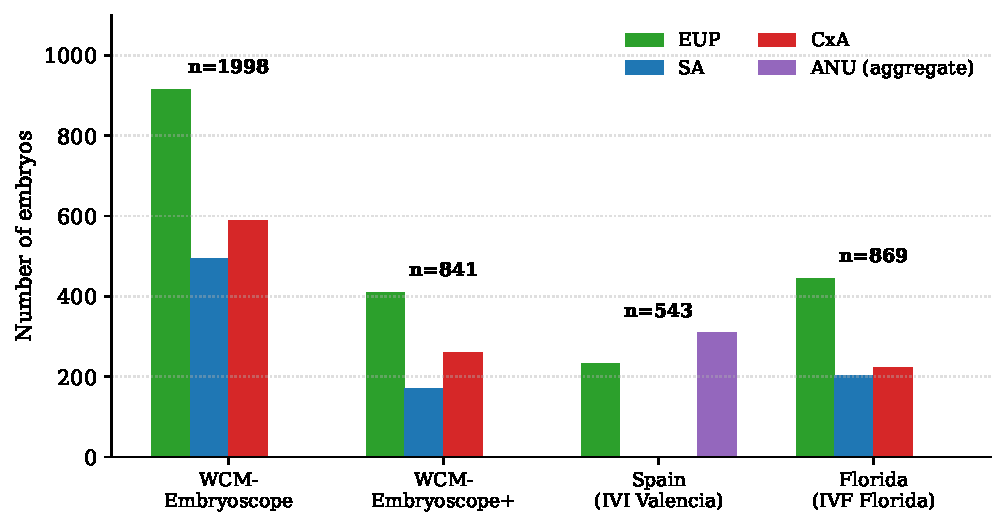
\includegraphics[width=0.72\textwidth]{figures/fig_datasets.pdf}
\caption{Characteristics of the four datasets used in this study. WCM-Embryoscope
(1{,}998 embryos), WCM-Embryoscope+ (841 embryos), Spain/IVI Valencia
(543 embryos), and Florida/IVF Florida (869 embryos). The Spain dataset reports
aneuploidy as a single aggregate class (ANU), while WCM and Florida report
single aneuploid (SA) and complex aneuploid (CxA) subcategories in addition
to euploid (EUP).}
\label{fig:datasets}
\end{figure}


% ---------- 2.2 Blastocyst Score Prediction ----------
\subsection{Blastocyst Score Prediction}

A central design choice in BELA is the use of blastocyst score as an interpretable intermediate representation that bridges raw time-lapse features and the downstream ploidy classifier. Predicting blastocyst score from video features, rather than predicting ploidy directly, allows the model to leverage a well-characterized label that has been shown to correlate with implantation success, euploidy, and live birth. Because the blastocyst score comprises three sub-components---inner cell mass (ICM), trophectoderm (TE), and expansion---we hypothesized that jointly predicting all four quantities through multitask learning would provide a regularizing signal that improves the primary prediction.

To test this hypothesis, we trained a multitask bidirectional LSTM on the WCM-Embryoscope training set to concurrently predict ICM score, TE score, expansion score, and the overall blastocyst score from 512-dimensional VGG16 feature vectors extracted from day-5 frames (96--112 hpi). Performance was measured using mean absolute error (MAE) between the model-derived blastocyst score (MDBS) and the embryologist-assigned ground-truth score. The multitask configuration achieved an MAE of $1.855 \pm 0.03$, compared with $1.877 \pm 0.027$ for a single-task variant that predicted blastocyst score alone, confirming that the auxiliary sub-score tasks provide a modest but consistent improvement (Figure~\ref{fig:mae_comparisons}, left panel). Both configurations exhibited moderate Pearson correlations (${>}0.7$) between predicted and actual scores on both the training and test partitions.

These results demonstrate that a temporal deep-learning model can approximate embryologist grading with reasonable fidelity from day-5 frames alone, without access to the additional time points that embryologists routinely consider. The interpretability of the intermediate blastocyst score is a practical advantage: clinicians can inspect the MDBS alongside the ploidy probability, providing a transparent basis for downstream decisions. Having established that blastocyst score can be reliably predicted, we next examined how the resulting MDBS performs as a feature for ploidy classification.

% -- Figure: MAE --
\begin{figure}[htbp]
\centering
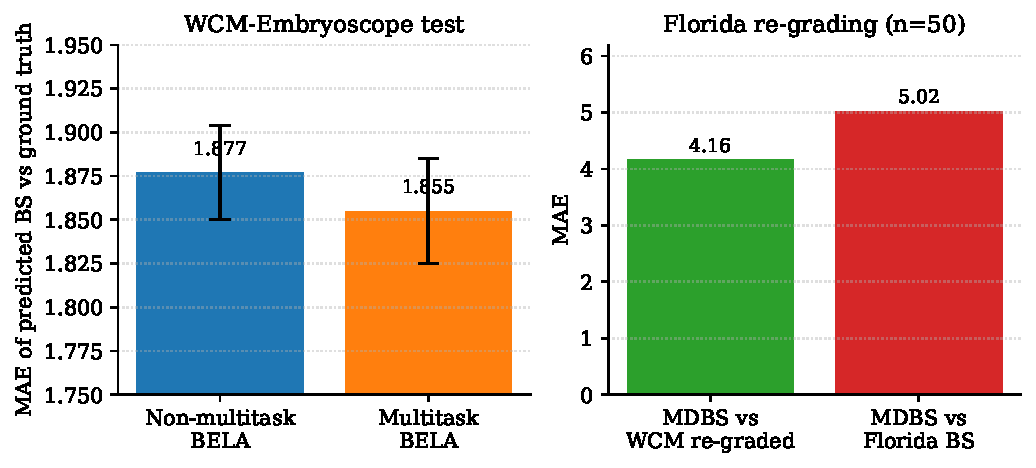
\includegraphics[width=0.95\textwidth]{figures/fig_mae_comparisons.pdf}
\caption{(Left) Mean absolute error (MAE) of predicted blastocyst score on
the WCM-Embryoscope test set for multitask BELA (1.855~$\pm$~0.03) and
non-multitask BELA (1.877~$\pm$~0.027). (Right) MAE between the model-derived
blastocyst score (MDBS) and two reference scores on 50 Florida embryos where
the MDBS deviated most strongly from the provided Florida blastocyst scores:
MDBS vs the Weill Cornell re-graded BS (4.16) and MDBS vs the original Florida
BS (5.02).}
\label{fig:mae_comparisons}
\end{figure}


% ---------- 2.3 Ploidy Classification WCM ----------
\subsection{Ploidy Classification on WCM Datasets}

The primary evaluation of BELA's ploidy discrimination was conducted on the WCM-Embryoscope test set, with the WCM-Embryoscope+ cohort serving as a held-out temporal validation set collected on a different imaging instrument. Two classification tasks were defined: euploid versus all aneuploid (EUP vs ANU) and euploid versus complex aneuploid (EUP vs CxA), the latter isolating the clinically more consequential category of multi-chromosomal abnormalities.

On the WCM-Embryoscope test set, BELA achieved an AUC of $0.66 \pm 0.008$ for the EUP vs ANU task without maternal age, which rose substantially to $0.76 \pm 0.002$ when maternal age was included as a covariate (Figure~\ref{fig:auc_wcm}). For the EUP vs CxA task, the corresponding AUC values were $0.708 \pm 0.004$ without age and $0.826 \pm 0.004$ with age. Across all tested scenarios---both tasks, both test sets, and both with and without maternal age---BELA significantly outperformed the day-5 video baseline, which directly predicts ploidy from BiLSTM features without the intermediate blastocyst-score step ($p < 0.05$, Student's $t$-test with Bonferroni correction).

The comparison with the embryologist-annotated blastocyst-score model is more nuanced and reveals the complementary value of maternal age. Without maternal age, the embryologist-annotated BS model surpassed BELA ($p < 0.05$) in all tasks except EUP vs ANU on the WCM-Embryoscope test set, where the two models were statistically comparable. This is expected, because the ground-truth BS inherently contains more precise morphological information than a model-derived approximation. However, when maternal age was incorporated, BELA outperformed the embryologist-annotated BS model on the WCM-Embryoscope test set ($p < 0.05$), indicating that the MDBS captures complementary age-related variation that the embryologist score alone does not encode. On the WCM-Embryoscope+ dataset, the embryologist-annotated model retained a slight advantage even with age, which may reflect differences in scoring consistency between the two imaging platforms. A summary of BELA's AUC performance across both tasks and age conditions is provided in Table~\ref{tab:auc_wcm}.

An additional observation emerged from the analysis of single aneuploid (SA) embryos within the EUP vs CxA classification framework. BELA predicted SA embryos approximately evenly as either euploid or complex aneuploid, suggesting that single aneuploid embryos occupy a morphological middle ground between these two classes and are correspondingly difficult to classify. This finding is consistent with dedicated EUP vs SA models, which yielded lower discrimination than the EUP vs CxA task, confirming that single chromosomal abnormalities produce subtler phenotypic signatures than complex ones. On the WCM-Embryoscope+ dataset, BELA demonstrated particularly strong recall for euploid embryos, indicating substantial potential for correctly identifying embryos suitable for transfer. These findings motivated us to investigate whether the same pattern holds in clinically independent external cohorts.

% -- Table: AUC Performance --
\begin{table}[htbp]
\centering
\caption{BELA AUC performance on the WCM-Embryoscope test set for the two ploidy classification tasks, with and without inclusion of maternal age.}
\label{tab:auc_wcm}
\begin{tabular}{lcc}
\toprule
Task & AUC without age & AUC with age \\
\midrule
EUP vs ANU & $0.66 \pm 0.008$ & $0.76 \pm 0.002$ \\
EUP vs CxA & $0.708 \pm 0.004$ & $0.826 \pm 0.004$ \\
\bottomrule
\end{tabular}
\end{table}

% -- Figure: AUC WCM --
\begin{figure}[htbp]
\centering
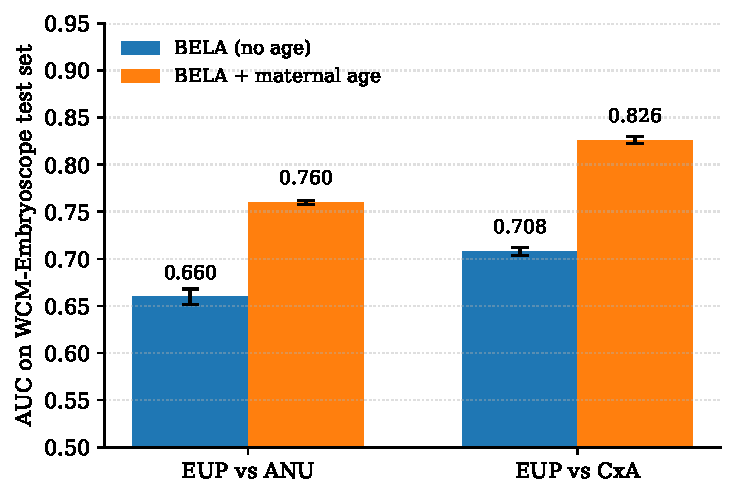
\includegraphics[width=0.72\textwidth]{figures/fig_auc_wcm.pdf}
\caption{BELA ploidy classification AUC on the WCM-Embryoscope test set with
and without inclusion of maternal age. For the EUP~vs~ANU task, AUC rises from
0.66~$\pm$~0.008 to 0.76~$\pm$~0.002 when maternal age is included. For the
EUP~vs~CxA task, AUC rises from 0.708~$\pm$~0.004 to 0.826~$\pm$~0.004.
Error bars denote standard errors across cross-validation folds.}
\label{fig:auc_wcm}
\end{figure}

% -- Figure: Pipeline Overview --
\begin{figure}[htbp]
\centering

\includegraphics[width=0.95\textwidth]{figures/fig_pipeline.pdf}
\caption{Overview of the BELA pipeline. Day-5 time-lapse frames (96--112 hpi)
are processed into 512-dimensional feature vectors by a pre-trained VGG16
backbone. A multitask bidirectional LSTM jointly predicts inner cell mass
(ICM), trophectoderm (TE), expansion score, and the overall blastocyst score.
The resulting model-derived blastocyst score (MDBS) is combined with maternal
age in a logistic regression to predict ploidy status.}
\label{fig:pipeline}
\end{figure}


% ---------- 2.4 External Validation ----------
\subsection{External Validation: Spain and Florida Cohorts}

Generalizability across clinical sites is a prerequisite for any model intended for deployment in diverse IVF settings. The Spain and Florida datasets provided two distinct external validation opportunities, each with its own challenges for cross-site transfer.

The Spain cohort from IVI Valencia comprised 543 embryos with aggregate EUP/ANU labels but without SA/CxA stratification or embryologist-derived blastocyst scores. Importantly, embryos in this cohort were artificially hatched on day 3, a procedure that produces bleached zona pellucida and reduced expansion compared with the WCM training data. PCA-based visualization of VGG16 feature encodings averaged across day-5 frames confirmed that the Spain data clustered distinctly from the WCM and Florida datasets, consistent with these procedural differences (Figure~\ref{fig:pca_placeholder}). Despite this distributional shift, BELA significantly outperformed the day-5 video model on the Spain dataset for the EUP vs ANU task in both conditions---with and without maternal age ($p < 0.05$). Notably, BELA's performance without maternal age remained comparable to its performance on the WCM datasets, suggesting that the model captures morphological features of ploidy that generalize across hatching protocols. When maternal age was included, performance decreased relative to the WCM results, likely reflecting demographic differences between the two patient populations: IVF is more affordable and accessible in Spain than in the United States, leading to different maternal-age distributions.

The Florida cohort from IVF Florida presented a different challenge. This dataset included 869 embryos with full SA/CxA/EUP stratification and embryologist-derived blastocyst scores, but the correlation between both blastocyst score and maternal age with ploidy was weaker than in the WCM data, and the blastocyst scores were concentrated around a score of 7, reducing the discriminative granularity of this feature. This loss of granularity likely stems from the fact that IVF Florida evaluates blastocysts at 115 and 144 hpi, rather than at the earlier time points used at WCM. As a result, performance of all models---including BELA---declined on this dataset relative to the WCM and Spain cohorts.

An encouraging finding from the Florida analysis was that the MDBS showed a stronger point-biserial correlation with ploidy status ($-0.119$) than the embryologist-derived blastocyst score ($-0.101$), indicating that BELA produces a score mapping more aligned with chromosomal status than the manual grading rubric used at this site. To corroborate this observation, an embryologist at WCM re-graded the 50 Florida embryos where the MDBS deviated most from the Florida-assigned scores. The MAE between the MDBS and the WCM re-graded score was 4.16, compared with 5.02 between the MDBS and the original Florida score (Figure~\ref{fig:mae_comparisons}, right panel), indicating greater agreement between the automated score and the WCM grading standard. This improved score alignment is likely the mechanism by which BELA, with maternal age included, significantly outperformed the model trained on maternal age and embryologist-derived blastocyst score for the EUP vs ANU task on the Florida dataset ($p < 0.05$). These cross-site analyses demonstrate that while absolute performance varies with local protocols and patient demographics, the relative advantage of BELA's automated scoring over both direct video classification and site-specific manual grading is maintained.

% -- Figure: PCA placeholder --
\begin{figure}[htbp]
\centering
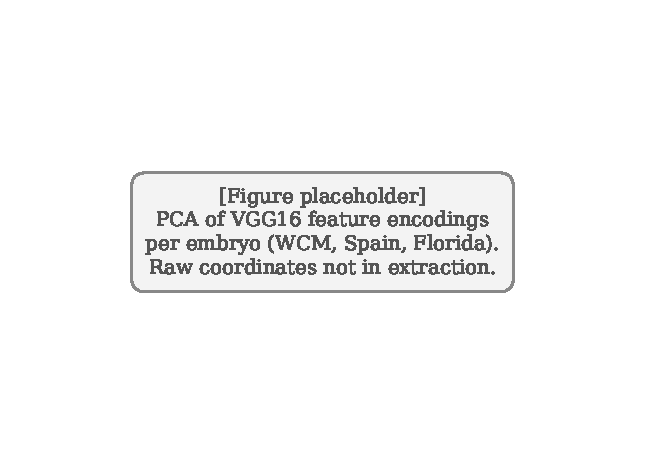
\includegraphics[width=0.5\textwidth]{figures/fig_pca_placeholder.pdf}
\caption{Schematic placeholder for PCA of VGG16 feature encodings of day-5
embryo frames (96--112 hpi) across the WCM-Embryoscope, WCM-Embryoscope+,
Spain, and Florida datasets. Per-embryo coordinates were not available in
the extracted materials used for this manuscript.}
\label{fig:pca_placeholder}
\end{figure}


% ---------- 2.5 STORK-V Deployment ----------
\subsection{STORK-V Clinical Deployment}

Translating a trained model into a tool that embryologists can use in daily practice requires a deployment infrastructure that is fast, accessible, and interpretable. To meet these requirements, we developed STORK-V, a web-based application that encapsulates the full BELA pipeline---from raw time-lapse input to ploidy probabilities and intermediate quality scores---in a single user-facing interface.

The STORK-V platform accepts time-lapse images captured between 96 and 112 hpi together with maternal age, and returns predictions from two models: one trained to discriminate EUP from ANU and another trained to discriminate EUP from CxA. The output includes probabilities for euploidy, aneuploidy, and complex aneuploidy, as well as the intermediate MDBS and its sub-component scores, which embryologists can use for independent quality assessment. From a computational standpoint, inference for a single embryo requires $30 \pm 5$ seconds on the platform, making it compatible with routine clinical workflows. On the training side, logistic regression models require an average of $2.5 \pm 1.2$ seconds and BiLSTM models require $30.3 \pm 11$ minutes on consumer-grade hardware (Apple M1 with TensorFlow Metal), while the full BELA model trains in 5.23 minutes on a high-performance GPU (NVIDIA A40). These training and inference times are summarized in Table~\ref{tab:timing}.

The availability of the STORK-V platform lowers the barrier to adoption in clinics that lack specialized computational infrastructure. Because the model requires no embryologist-derived annotation as input, it can be deployed at sites that do not routinely perform blastocyst scoring, thereby standardizing the assessment process across institutions. The interpretable intermediate scores further support clinician trust: rather than receiving an opaque ploidy probability, the user obtains a decomposed view of the embryo's predicted morphological quality alongside the classification output. Taken together, the results across all four cohorts and the practical deployment through STORK-V provide a foundation for evaluating the clinical impact and broader implications of this approach.

% -- Table: Timing --
\begin{table}[htbp]
\centering
\caption{Computational training and inference times for the components of the BELA pipeline and the STORK-V deployment platform.}
\label{tab:timing}
\begin{tabular}{lc}
\toprule
Component & Time \\
\midrule
Logistic regression training (M1 Mac) & $2.5 \pm 1.2$ s \\
BiLSTM training (M1 Mac) & $30.3 \pm 11$ min \\
Full BELA training (NVIDIA A40 GPU) & 5.23 min \\
Single-embryo inference (STORK-V) & $30 \pm 5$ s \\
\bottomrule
\end{tabular}
\end{table}


% ==========================================================================
% DISCUSSION
% ==========================================================================
\section{Discussion}

The results presented above demonstrate that BELA provides a fully automated, non-invasive approach to embryo ploidy prediction that is competitive with models relying on subjective embryologist annotation and consistently superior to direct video-based classification. By decomposing the ploidy prediction task into an interpretable blastocyst-score prediction step followed by a logistic regression, BELA combines the temporal richness of time-lapse imaging with the established clinical relevance of morphological grading, while eliminating the inter-observer variability that plagues manual scoring. The inclusion of maternal age as a covariate further enhances discriminative performance, reflecting the well-documented biological relationship between advancing maternal age and embryonic aneuploidy rates.

The performance of BELA can be situated within the broader landscape of deep-learning approaches to ploidy prediction. ERICA, operating on 1{,}231 static blastocyst images, achieved an AUC of 74\% for ploidy classification \citep{chavezbadiola2020erica}, while Lee et al.\ reported an AUC of 0.74 using an end-to-end two-stream inflated 3D model on 670 image sequences \citep{lee2021endtoend}. BELA's AUC of $0.76 \pm 0.002$ for EUP vs ANU and $0.826 \pm 0.004$ for EUP vs CxA on the WCM-Embryoscope test set (with maternal age) compares favorably with these benchmarks, while requiring only a narrowly defined 16-hour developmental window rather than the full time-lapse sequence or manually curated morphological features. The multitask learning formulation, which jointly predicts ICM, TE, expansion, and overall blastocyst score, contributed a modest but consistent reduction in MAE ($1.855 \pm 0.03$ vs $1.877 \pm 0.027$ for the single-task variant), suggesting that the shared structure among sub-scores provides useful inductive bias for the temporal model.

A key strength of this study is the multi-site validation design. Models trained exclusively on data from a single institution often fail to generalize when deployed in clinics with different patient demographics, embryo culture protocols, or imaging hardware. Our results on the Spain and Florida datasets illustrate both the promise and the challenges of cross-site transfer. On the Spain dataset, where embryos were artificially hatched on day 3 and exhibited morphological features absent from the training data, BELA nonetheless significantly outperformed the day-5 video baseline. On the Florida dataset, where blastocyst scores lacked the granularity observed in the WCM data, the MDBS from BELA correlated more strongly with ploidy ($-0.119$) than the embryologist-derived score ($-0.101$), and re-grading by a WCM embryologist confirmed better agreement between the MDBS and the WCM scoring standard (MAE of 4.16 vs 5.02). These findings suggest that BELA's automated scoring captures ploidy-relevant morphological features more reliably than manual grading rubrics that vary between sites. The comprehensive benchmark by Bamford et al.\ \citep{bamford2023ml12}, which evaluated twelve machine-learning models on a morphokinetic meta-dataset, underscores the difficulty of this generalization problem and reinforces the importance of multi-site validation.

An important distinction between this study and much prior work is the composition of the evaluation cohorts. Many earlier studies included non-viable embryos as negative examples, artificially inflating AUC values because such embryos are morphologically distinct from viable ones. In contrast, the datasets used here consist exclusively of good biopsied embryos---all of which reached blastocyst stage and underwent PGT-A---making the classification task substantially harder but also more clinically realistic. Within these cohorts, BELA's performance stratified by Society for Assisted Reproductive Technology (SART) maternal-age groups exhibited a bimodal pattern on the WCM-Embryoscope and WCM-Embryoscope+ datasets, with the highest discrimination observed in the youngest and oldest age brackets. This pattern is biologically plausible: younger patients have a higher baseline euploidy rate that may facilitate separation, while older patients have a higher aneuploidy prevalence that similarly aids discrimination. On the Spain and Florida datasets, this bimodal pattern was not replicated, likely reflecting demographic differences in IVF utilization across countries and the smaller sample sizes within individual age strata.

Several limitations related to data availability and model architecture should be acknowledged. The training set comprised approximately 2{,}000 time-lapse sequences from a single institution after exclusion criteria were applied, reducing the effective sample to 1{,}684 embryos for model development. This limited sample size precluded the exploration of more parameter-intensive architectures such as 3D convolutional networks or two-stream inflated convolutional models that have shown promise in other video understanding domains. Furthermore, despite evaluating multiple pre-trained feature extractors, the ImageNet-pretrained VGG16 architecture remained the best-performing option, and it is possible that domain-specific pretraining on embryo images---such as the recent IVF foundation model trained on 18 million time-lapse images \citep{rajendran2025femi}---could yield more informative representations from earlier developmental stages. Our models also did not incorporate hormonal data, demographic variables beyond maternal age, or other clinically relevant features that could further improve ploidy prediction.

Additional limitations stem from the labeling strategy and cohort composition. The use of blastocyst score as an intermediate label, while motivated by its established association with clinical outcomes, inherits the subjectivity of the original annotation and may introduce systematic bias if scoring practices differ between the training and deployment sites. The current pipeline also excludes mosaic embryos, which represent a clinically important subpopulation whose ploidy status falls between euploid and aneuploid; future work should address the identification and appropriate handling of mosaicism. Finally, the use of different NGS platforms for PGT-A across clinics introduces potential variability in ground-truth labels, as there is significant inter-laboratory variation in detection rates for single versus complex aneuploidy and no industry-wide standardization of PGT-A interpretation \citep{zou2022timelapse}. Differences in inclusion and exclusion criteria between datasets may also have contributed to the observed variation in model performance across test cohorts.

Looking forward, BELA exemplifies a design paradigm---automated intermediate representation followed by interpretable downstream classification---that could be extended in several clinically meaningful directions. Models that incorporate additional developmental time windows, multi-modal clinical data, or more expressive temporal architectures could further narrow the performance gap between non-invasive prediction and PGT-A. The STORK-V platform provides a practical deployment vehicle for such improvements and can serve as the basis for prospective clinical validation studies. Importantly, BELA is not intended to replace PGT-A but rather to provide a complementary, cost-effective, and accessible layer of information that supports embryologist decision-making. By preselecting embryos with higher odds of euploidy, BELA could reduce unnecessary biopsies, decrease the financial burden on patients, and ultimately contribute to improved IVF success rates. Automated blastocyst scoring via the MDBS also has standalone clinical value as a standardized, objective alternative to subjective manual grading, and future iterations of fully end-to-end models that dispense with manually curated features are well-positioned for integration into routine clinical workflows.


% ==========================================================================
% MATERIALS AND METHODS
% ==========================================================================
\section{Materials and Methods}

\subsection{Datasets and Clinical Annotations}

The WCM-Embryoscope dataset was collected at the Center for Reproductive Medicine at Weill Cornell Medicine between 2018 and 2019 and comprises time-lapse images and PGT-A results for 1{,}998 embryos (494 SA, 588 CxA, 916 EUP) from 498 patients, with an average of four biopsied embryos per patient. Each embryo's clinical record included an embryologist-derived blastocyst score (BS), morphokinetic parameters, and maternal age at the time of oocyte retrieval. The blastocyst score ranges from 3 to 14 (lower is better) and is computed as the sum of converted grades for expansion, ICM, and TE, with this formulation having been shown to be predictive of implantation success, euploidy, and live birth. The WCM-Embryoscope+ dataset (2019--2020) contained 841 embryos (170 SA, 261 CxA, 410 EUP) captured on the Embryoscope+ instrument with equivalent clinical annotations. The Spain dataset from IVI Valencia contained 543 embryos (309 ANU, 234 EUP) with time-lapse sequences, morphokinetic parameters, and maternal age but without SA/CxA stratification or BS. The Florida dataset from IVF Florida contained 869 embryos (202 SA, 222 CxA, 445 EUP) with maternal age and blastocyst scores. PGT-A was performed using next-generation sequencing (NGS) technology at each site \citep{garciapascual2020ngs}. At WCM, embryos were biopsied on day 5 or day 6 depending on when they reached the blastocyst stage, and biopsied trophectoderm cells were analyzed at the Ronald O.\ Perelman and Claudia Cohen Center for Reproductive Medicine. In the Spain dataset, embryos were subjected to assisted hatching on day 3 after cell counting, with trophectoderm biopsy performed at the blastocyst stage; analyses were conducted by Igenomix Spain using Thermo Fisher Scientific NGS technology. Florida embryos were also analyzed by Igenomix using the same NGS platform. Each sample was treated independently irrespective of parental origin.

\subsection{Temporal and Spatial Preprocessing}

Raw time-lapse sequences varied in length, frame rate, start point, and end point. To standardize them, we designated 301 time points at 0.5-hour intervals from 0 to 150 hpi. For each embryo, the frame captured closest to each standardized time point was assigned to that position; if no frame fell within a 2-hour imputation window, a blank frame was substituted. This protocol reduced variability in sequence length and ensured that all embryos were represented on a common temporal grid. For video classification tasks, subsequences were extracted using start, end, and interval parameters; for example, the day-5 input used start = 96 hpi, end = 112 hpi. Each frame was resized from $800 \times 800$ to $224 \times 224$ pixels, and a circle Hough Transform was applied for embryo segmentation to minimize background bias. Video augmentation comprised random horizontal flipping and random rotations, simulating real-world orientation variation while effectively expanding the training set. This preprocessing pipeline was uniformly applied across all four datasets.

\subsection{Feature Extraction}

Spatial features were extracted from each preprocessed frame using an ImageNet-pretrained convolutional neural network implemented in TensorFlow 2.7. We evaluated multiple pre-trained architectures as candidate feature extractors, including ResNet, InceptionV3, and DenseNet variants, in addition to VGG16. Each architecture was assessed by measuring the downstream performance of the BiLSTM blastocyst-score predictor trained on the extracted features. Across all tasks, the VGG16 architecture with ImageNet-pretrained weights consistently yielded the best downstream performance and was therefore selected for the final pipeline. The final average-pooling layer of VGG16 produced a 512-dimensional feature vector for each frame, providing a compact spatial representation that served as input to the temporal model.

\subsection{Multitask BiLSTM for Blastocyst Score Prediction}

The temporal feature sequences were processed by a bidirectional LSTM (BiLSTM) network comprising one bidirectional LSTM layer followed by two multi-unit dense layers. For each prediction task, a single-unit dense output layer was appended. The model was configured for multitask learning, jointly predicting blastocyst score, ICM score, TE score, and expansion score with equal loss weights for each task. Maternal age was included as an additional input feature in the BiLSTM regression model, concatenated with the temporal feature representation prior to the dense layers. Because all tasks are regression-based, we used logcosh as the loss function and Adam as the optimizer; early stopping with patience of 5 epochs was used, monitoring validation loss on the cross-fold partition. Alternative architectures incorporating attention mechanisms and multiple stacked bidirectional LSTM layers were explored but failed to improve performance significantly across all tasks ($p > 0.05$). The final model produced a model-derived blastocyst score (MDBS) for each embryo.

\subsection{Ploidy Classification via Logistic Regression}

The second step of BELA used the MDBS produced by the BiLSTM as the primary input feature for ploidy classification. A logistic regression model was trained with cross-entropy loss for each binary classification task (EUP vs ANU and EUP vs CxA). In the age-inclusive configuration, maternal age at oocyte retrieval was included as an additional continuous covariate alongside the MDBS, allowing the classifier to exploit the well-documented relationship between advancing maternal age and increased aneuploidy risk. Each logistic regression model was trained on the MDBS values produced by the corresponding cross-validation fold of the BiLSTM, and performance metrics were averaged across all four folds to yield the final estimates.

\subsection{Training Protocol and Cross-Validation}

Only the WCM-Embryoscope data were used for training. Embryos failing exclusion criteria (absent from petri dish, less than half-visible, or too dim) were removed, reducing the dataset from 1{,}998 to 1{,}684 embryos. The data were split 70/30 for training and testing. Four-fold cross-validation was employed for BiLSTM training, and a separate logistic regression was trained on each fold's predicted blastocyst scores. Performance metrics (accuracy, AUC, precision, recall) were averaged across folds. Two baselines were trained on the same cross-validation splits: a day-5 video model that directly predicts ploidy from BiLSTM features (96--112 hpi), and an embryologist-annotated model that uses the ground-truth BS in a logistic regression.

\subsection{Statistical Analysis}

Group comparisons were performed using the Student's $t$-test, selected because the data were approximately normally distributed with similar variances between groups. All comparisons were adjusted for multiple testing using Bonferroni correction.


% ==========================================================================
% REFERENCES
% ==========================================================================
\bibliographystyle{plainnat}
\bibliography{references}

\end{document}
